\chapter{Desenvolvimento do Projeto}

O projeto do sistema de iluminação controlado pela internet foi desenvolvido com o objetivo de apresentar determinadas funcionalidades e demonstrar a potencialidade de economia de energia. As funcionalidades propostas foram as de, remotamente, ligar e desligar a iluminação; apresentar dois modos de controle da luminosidade: O modo normal no qual o usuário poderá escolher a intensidade da fita de LED e o modo econômico no qual o sistema levará em conta a iluminação ambiente para manter um nível mínimo, definido pelo usuário, de luminosidade. 

O planejamento do esquema eletrônico foi norteado pelo microcontrolador escolhido e pelas funcionalidades propostas. A descrição dos elementos físicos usados no projeto da lâmpada inteligente pode ser resumida pelo esquema geral do projeto na Figura \ref{esquema}.

\begin{figure}[ht]
    \begin{center}
    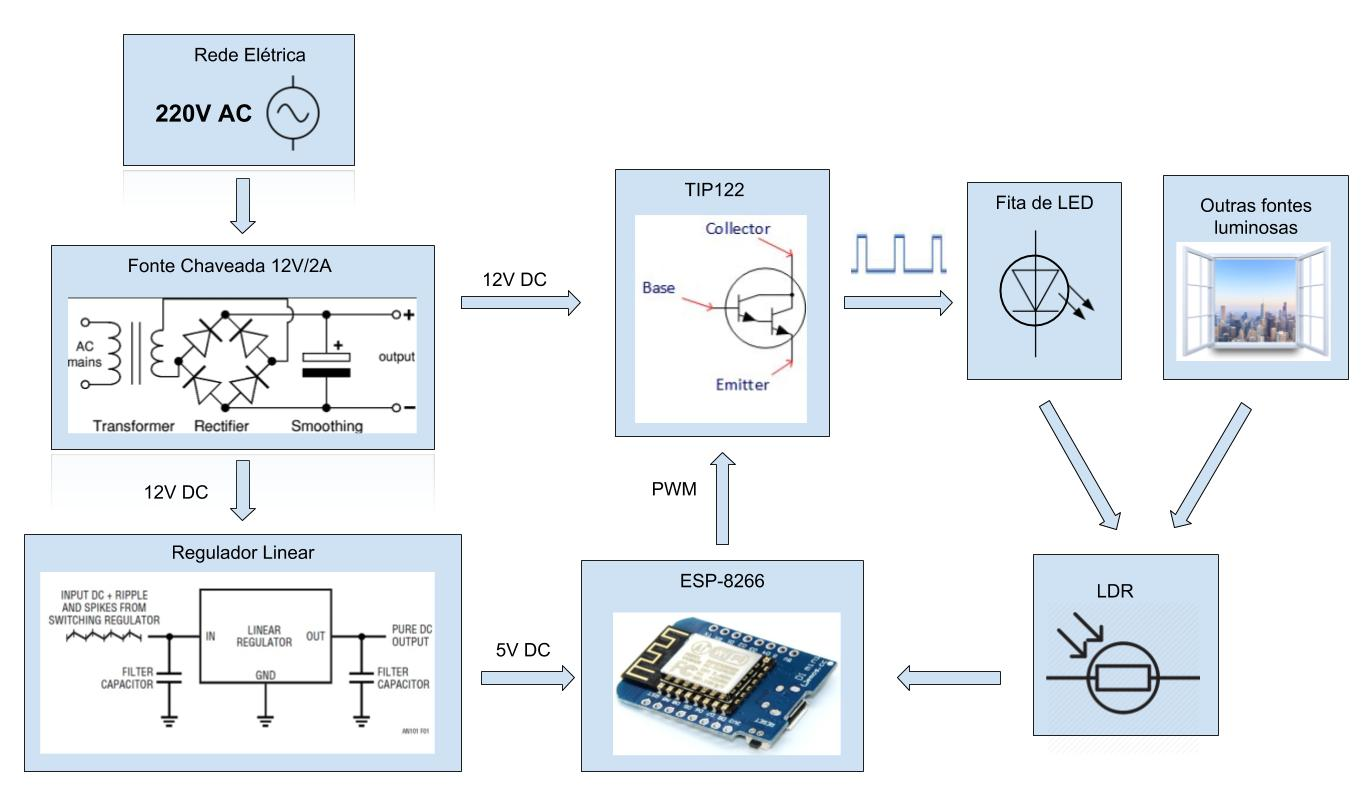
\includegraphics[width=\textwidth]{figuras/esquema_eletrico.jpg}
    \end{center}
    \caption[Esquema geral do projeto da fita de LED MQTT.]{Esquema geral do projeto da fita de LED MQTT.}
    \label{esquema}
\end{figure}

O modo econômico é baseado no controle automático da intensidade luminosa do ambiente em questão considerando a contribuição da fita de LED e de outras fontes de iluminação. O sistema de controle é realimentado pelo sensor de luminosidade, um resistor dependente de luz cujo valor de resistência diminui com o aumento da intensidade luminosa. O controlador escolhido para o sistema é controlador \acf{PID}. A saída do controlador é tratada como a duração do ciclo ativo do sinal digital que ``chaveia'' a potência da fita de LED.

A demonstração da economia de energia do sistema é baseada na comparação das estimativas do consumo da iluminação com intensidade máxima e do consumo com intensidade controlada automaticamente.

\section{Funcionalidades}

\subsection{Ligar e Desligar}

O sistema deve ser capaz de ligar e desligar a iluminação de LED por meio da internet, para isso o sistema de iluminação deve se comunicar com as interfaces de usuário, aplicativo móvel e página \textit{web}, e essas têm que manter sincronia desta informação. O tópico MQTT ``\texttt{/feeds/onoff}'' foi criado para que as interfaces possam publicar comandos para ligar e desligar, e para que possam subscrever as informações publicadas para que, caso uma das interfaces publique um comando a outra interface possa sincronizar-se e mostrar o novo estado para o usuário.

\subsection{Ajuste Manual da Iluminação}

O modo manual de ajuste é caracterizado pela escolha arbitrária da intensidade da fita de LED pelo usuário. A escolha de um valor inteiro de 0 a 100, que deve representar a porcentagem da intensidade máxima da iluminação, é feita por meio de ambas as interfaces ao publicar no tópico ``\texttt{/feeds/pwmin}'' o valor da intensidade. Assim como no ligamento/desligamento as interfaces também subscrevem esse tópico para manter a informação sincronizada. A seleção do modo de funcionamento é controlado através do tópico ``\texttt{/feeds/modo}''.

\subsection{Ajuste Automático}

O modo automático de ajuste consiste no controle da luminosidade pelo sistema com a referência de ajuste, ou ``\textit{setpoint}'', escolhida pelo usuário pelo modo manual e com o sinal de realimentação medido por meio do  resistor dependente de luz (LDR). O controlador usado na malha fechada de controle da iluminação é o \acf{PID}. A referência de controle é a tensão medida no LDR no momento que o usuário muda o modo de operação, do modo ``Manual'' para o modo ``Econômico''. O sistema deve controlar a intensidade da fita de LED de modo que, combinada com a iluminação ambiente, o sistema possa manter a iluminação no nível escolhido pelo usuário.

\section{Materiais}

\subsection{Alimentação}

A fonte de alimentação elétrica do projeto é uma fonte comercial de 12V/1A de padrão comercial “\textit{bivolt}” com plugue P4. Os 12V fornecidos pela fonte serão partilhados pela fonte de iluminação e pelo sistema embarcado. Um regulador baseado no CI AMS1117 será usado para transformar os 12V da fonte em 5V para alimentar o sistema com o microcontrolador. Esse regulador pode fornecer até 1A que já é mais que o suficiente para o ESP-8266 que consome em torno de 220 mA durante curtos períodos quando está transmitindo via WiFi.

\subsection{Módulo Microcontrolador}

Como mencionado, o microcontrolador escolhido para o projeto é o ESP-8266 que inclui capacidade de comunicação WiFi. A própria fabricante do CI comercializa alguns módulos que facilitam o desenvolvimento com o ESP-8266 com antenas, LED, memória \textit{flash} e outros periféricos. Um desses módulos, o ESP-12 é usado por diversas empresas para fabricarem seus kits de desenvolvimento com ainda mais facilidades para o desenvolvedor. O kit usado neste projeto é “\textit{Wemos D1 Mini}” que conta com conversor USB-serial, regulador de tensão para transformar os 5V DC provenientes da porta ``USB'' ou da alimentação externa para os 3.3V DC que o ESP-8266 demanda, oscilador, botão para \textit{reset} e conectores para os pinos de entrada e saída.

\begin{table}
    \centering
    \label{wemos_dados}
    \caption{Especificações do kit \textit{Wemos D1 Mini}}
    \begin{tabular}{ll} 
        \hline
        Kit de desenvolvimento          & Wemos D1 Mini  \\ 
        \hline
        SoC                             & ESP-8266       \\ 
        \hline
        Pinos de I/O digitais           & 11             \\ 
        \hline
        Entradas analógicas             & 1 (3,2V máx)   \\ 
        \hline
        Clock                           & 80 MHz         \\ 
        \hline
        Memória \textit{flash}          & 4 MB           \\
        \hline
    \end{tabular}
\end{table}

O pino de entrada analógica do módulo usado tem uma tensão máxima especificada de 3,2V, apesar de a tensão máxima de entrada do ESP-8266 ser de 1V segundo suas características elétricas \cite{esp}. Isto se deve ao fato de o módulo ``\textit{Wemos D1 Mini}'' apresentar um divisor de tensão conectado ao pino de entrada analógica do SoC fazendo com que a tensão aplicada a este pino seja mapeada de um intervalo de, 0 a 3,2V no devido pino do módulo, para um intervalo de 0 a 1V no pino do ESP-8266.

\begin{figure}[ht]
    \begin{center}
    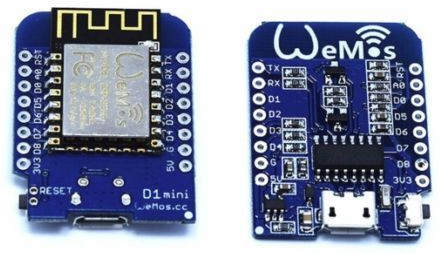
\includegraphics[width=0.4\textwidth]{figuras/wemos.PNG}
    \end{center}
    \caption[Ilustração do módulo \textit{Wemos D1 Mini}.]{Módulo \textit{Wemos D1 Mini} baseado no ESP-8266 visto de cima e de baixo.}
    \label{wemos}
\end{figure}

\subsection{Sensor de Luminosidade}

O sensor de luminosidade é um ``fotoresistor'' ou \acf{LDR} cuja resistência, geralmente, diminui com o aumento da intensidade luminosa linearmente. Geralmente são materiais semicondutores de alta resistividade, mas que quando expostos à luz, têm elétrons liberados em sua camada de condução aumentando assim sua condutividade por isso são geralmente chamados de células fotocondutivas. Existem LDRs sensíveis a faixas de radiação ultravioleta, infravermelho e a luz visível, que são os mais comuns.

O LDR usado \cite{ldr} é feito do material semicondutor CdS e apresenta uma curva de resistência em função da intensidade luminosa como mostrada na Figura \ref{reta}. Os valores mostrados podem variar um pouco com a temperatura e existe um comportamento transiente da ordem de 10 ms de duração, o que não se torna relevante para medições menos frequentes que uma repetição por minuto, por exemplo.

\begin{figure}[htb]
    \begin{center}
    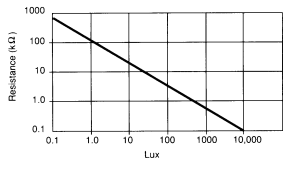
\includegraphics[width=0.4\textwidth]{figuras/reta.PNG}
    \end{center}
    \caption[Gráfico da reisitência \textit{versus} intensidade luminos do LDR.]{Gráfico da reisitência \textit{versus} intensidade luminos do LDR.}
    \label{reta}
\end{figure}

\subsection{Fita de LED}

A fonte de iluminação é uma fita de LED branca que consiste de elementos de três LEDs e um resistor em série para limitar a corrente, com vários desses elementos ligados em paralelo o que permite que todos os elementos sejam submetidos à mesma tensão e que a fita possa ser cortada em determinados pontos e continue funcionando. A fita de LED adquirida para o projeto tem as especificações listadas na Tabela 3.2.

\begin{figure}[htb]
    \begin{center}
    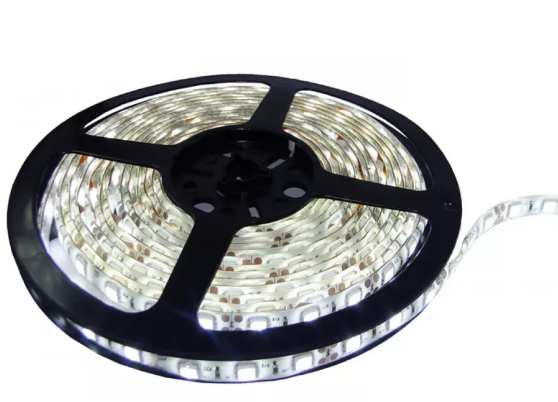
\includegraphics[width=0.3\textwidth]{figuras/fitaled.PNG}
    \end{center}
    \caption[Ilustração da fita de LED branca.]{Ilustração da fita de LED de cor branca fria de 12V.}
    \label{fitaled}
\end{figure}

 

\begin{table}[hbt]
    \centering
    \label{fitaled_dados}
    \caption{Especificações da fita de LED branca}
    \begin{tabular}{ll} 
        \hline
        Tensão de Operação (V)  & 12            \\ 
        \hline
        Consumo por metro (W/m) & 4.8           \\ 
        \hline
        Comprimento (m)         & 5             \\ 
        \hline
        LEDs por metro          & 60            \\ 
        \hline
        Temperatura da cor (K)  & 6000(frio)    \\
        \hline
    \end{tabular}
\end{table}

O controle da luminosidade será feito por chaveamento da alimentação da fita de LED com \acf{PWM}, técnica que permite controlar digitalmente a potência entregue a atuadores ao determinar a parcela do período em nível lógico alto, de um sinal alternado. O microcontrolador irá chavear um transistor \textit{darlington} “TIP122” \cite{tip122}.

\section{Ferramentas}

\subsection{\textit{Broker} MQTT}

O \textit{broker}, ou servidor, MQTT responsável pelo controle das mensagens intercambiadas na rede será o \textit{broker} da ``\textit{Adafruit}'' \cite{adafruit}. O serviço oferecido pela \textit{Adafruit} conta com um  \textit{broker} MQTT configurado com níveis de QoS 0 e 1, tópicos especiais como o ``\texttt{time/seconds}'' que fornece um número de segundos passados desde primeiro de janeiro de 1970 (\textit{Unix Time}) ou o tópico ``\texttt{(username)/throttle}'' que indica se a limitação de frequência de publicações foi atingida (que na versão grátis do serviço é de 30 vezes por minuto). O seviço da \textit{Adafruit} fornece também uma biblioteca da MQTT própria para \textit{Arduino} que define várias funções de \textit{callback} de subscrições e rotinas de conexão, desconexão e outras.

Uma interface de controle e visualização \textit{web} também é fornecida pela \textit{Adafruit} com possibilidade de implementação de botões, mostradores de valores, gráficos em tempo real, entre outras funcionalidades.

\subsection{Ambiente de Desenvolvimento de \textit{Software}}

O ESP-8266 possui um conjunto de bibliotecas e ferramentas, cujo objetivo é produzir código que, quando compilado, pode ser gravado na memória de programa e executado. Essas ferramentas levam o nome de ``SDK'' (\textit{Software Development Kit}) e são fornecidas, oficialmente, pela fabricante \textit{Espressif}. Uma comunidade de desenvolvedores do ESP-8266 criou uma estrutura de interfaces e adaptações (\textit{framework}) de código aberto para a SDK oficial para que fosse possível programar com a linguagem ``C++'' e usar as bibliotecas do \textit{Arduino}.

O desenvolvimento do software foi feito na IDE (\textit{Integrated Development Environment}) ``\textit{Visual Studio Code}'' da ``\textit{Microsoft}'' que é essencialmente um editor de texto de código aberto, muitas opções de customização e capacidade de conexão com extensões de terceiros. Uma dessas extensões foi usada, o ``PlatformIO'', Figura \ref{pio}, que é uma plataforma que conta com compiladores e outras ferramentas de diversos microcontroladores como \textit{Arduino}, ARM, \textit{Atmel} e vários outros. A extensão conta ainda com terminal virtual, monitor de porta serial, ferramentas de depuração de código e suporte à versionamento de código online.

\begin{figure}[ht]
    \begin{center}
    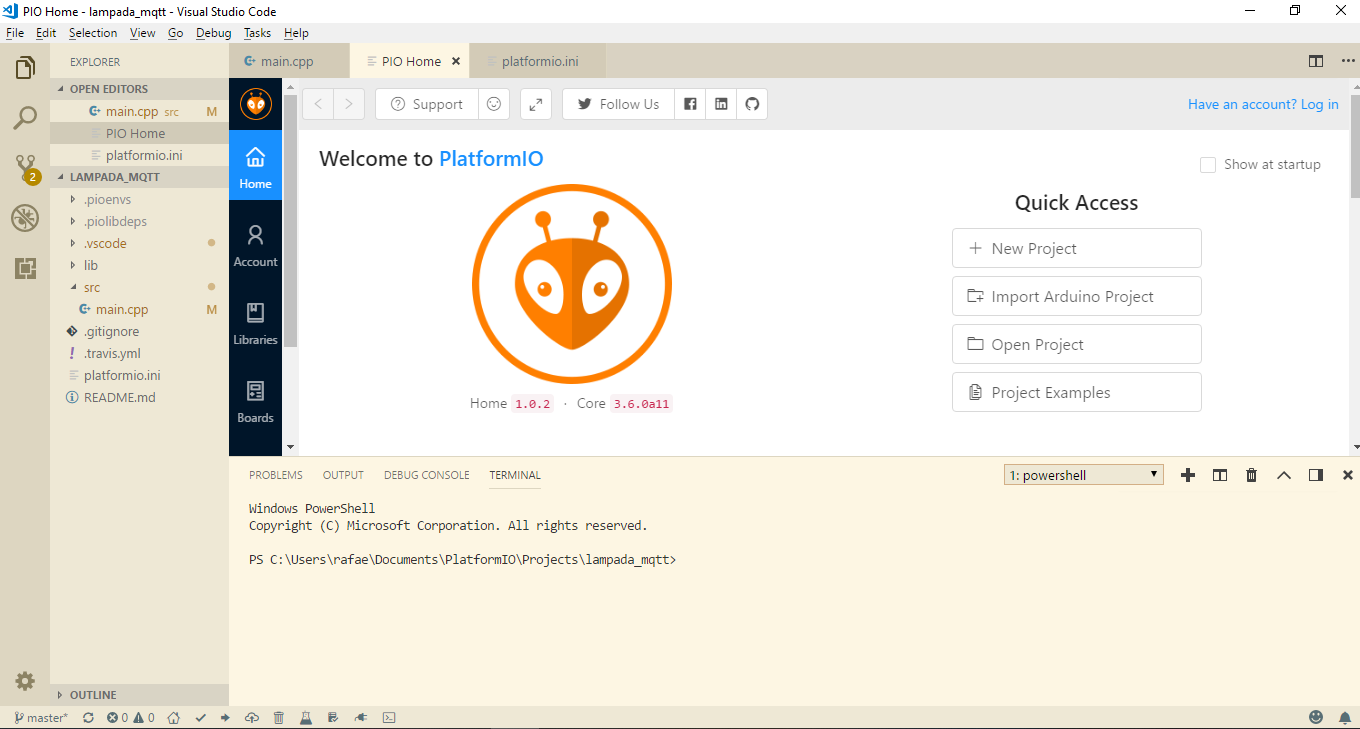
\includegraphics[width=\textwidth]{figuras/pio.PNG}
    \end{center}
    \caption[Ilustração do Visual Studio Code com o PlatformIO.]{Ilustração do ambiente de desenvolvimento ``Visual Studio Code'' com a extensão ``PlatformIO''.}
    \label{pio}
\end{figure}

\subsection{Bibliotecas}

Como mencionado, a programação foi feita na linguagem de programação ``C++'' com algumas bibliotecas de terceiros. A primeira a ser mencionada é a biblioteca do \textit{Arduino} que disponibiliza várias funções e definições que permitem uma grande simplicidade legibilidade do código escrito \cite{arduino}.

Outra biblioteca usada foi ``Esp8266WiFi'' \cite{espwifi}que disponibiliza várias rotinas relativas a conexão do ESP-8266 como a rede WiFi, reconexão, códigos relativos a camada TCP/IP e outros detalhes importantes para que o uso da internet com o microcontrolador seja possível.

A biblioteca ``WiFi \textit{Manager}'' \cite{wifimng} foi também usada e permitiu automatizar e generalizar o processo de autenticação do projeto para qualquer rede WiFi por meio da criação de uma página \textit{web} pela qual o usuário pode escolher a rede desejada e informar sua senha para que o ESP-8266 se conecte e salve essas informações em caso de reconexão.

\section{Metodologia}

Dadas as funcionalidades e características desejadas para o sistema, e os materiais e ferramentas, serão descritos agora os procedimentos e métodos na produção do arranjo físico, eletrônico do projeto, do firmware do microcontrolador e configuração das interfaces.

\subsection{Montagem}

Os principais componentes e materiais usados no projeto já foram descritos no capítulo 3. O esquema elétrico foi pensado com o objetivo de fazer com que o sistema atendesse às funcionalidades propostas.

% FIGURA NO FRITZING DA PROTOBOARD
\begin{figure}[ht]
    \begin{center}
    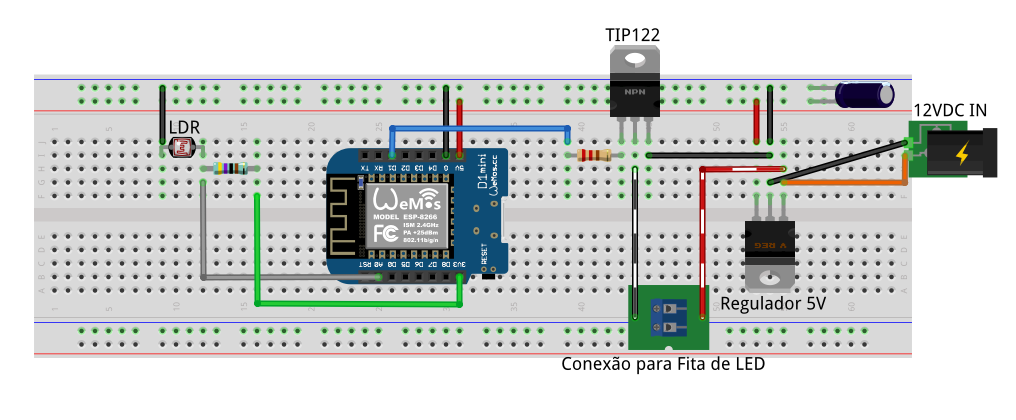
\includegraphics[width=\textwidth]{figuras/fritzproto.PNG}
    \end{center}
    \caption[Ilustração da placa de circuito protótipo do sistema de iluminação.]{Ilustração da placa de circuito protótipo do sistema de iluminação.}
    \label{fproto}
\end{figure}

A lista completa de materiais usados no projeto é detalhada na tabela \ref{BOM}.

\begin{table}
    \centering
    \caption{Lista de materiais}
    \label{BOM}
    \begin{tabular}{ll} 
        \hline
        Material                                                       & Quantidade  \\ 
        \hline
        \hline
        Fonte de chaveada 220VAC \textasciitilde{} 12VDC/2A            & 1           \\ 
        \hline
        Kit de regulador para \textit{protoboard} baseado no CI LM1117 & 1           \\ 
        \hline
        \textit{Wemos~}D1 Mini                                         & 1           \\ 
        \hline
        Fita de LED branca 3528 12V 4.8W/m                             & 1           \\ 
        \hline
        Sensor de Luminosidade LDR 5mm                                 & 1           \\ 
        \hline
        TIP122 Transistor \textit{Darlington} NPN                      & 1           \\ 
        \hline
        Resistor $4,7K\Omega$                                          & 1           \\ 
        \hline
        Resistor $220\Omega$                                           & 1           \\ 
        \hline
        Conector P4 macho                                              & 1           \\
        \hline
        Conector P4 fêmea                                              & 1           \\
        \hline
    \end{tabular}
\end{table}

O esquema eletrônico dos componentes é mostrado na Figura \ref{fsch} e ilustrado na Figura \ref{fproto} conforme montado na \textit{protoboard}.

\begin{figure}[ht]
    \begin{center}
    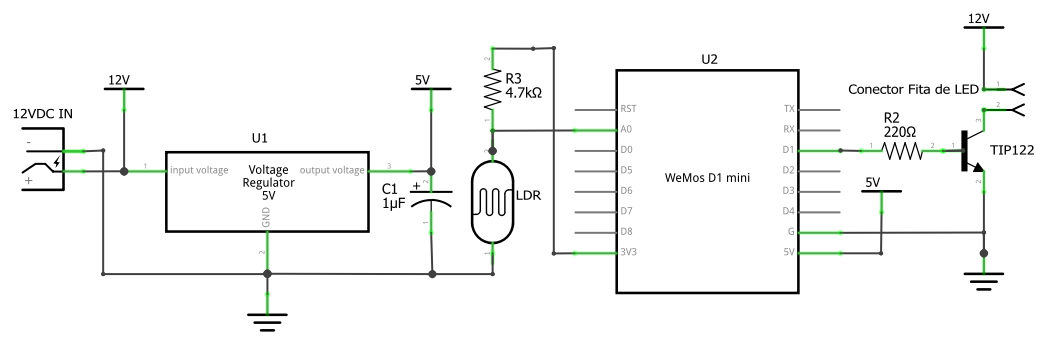
\includegraphics[width=\textwidth]{figuras/fritzsch.PNG}
    \end{center}
    \caption[Ilustração do esquemático eletrônico do circuito do sistema de iluminação.]{Ilustração do esquemático eletrônico do circuito do sistema de iluminação.}
    \label{fsch}
\end{figure}

O pino de entrada analógico do \textit{Wemos D1 Mini} suporta tensões de 0 a 3,2V. O conversor analógico-digital neste pino tém resolução de 10 \textit{bits} e, por isso, apresenta resolução de 1024 níveis de tensão igualmente espaçados cada um com aproximadamente 3 mV.

\begin{equation}
    \label{eq:pj_1}
    \Delta V = \frac{3,2}{2^{10}} = 0,003125 V \simeq 3 mV
\end{equation}

O divisor de tensão no LDR (o resistor de $4,7K\Omega$ entre a referência de 3.2V e o pino de entrada analógico, e o LDR entre este pino e o referencial de terra) faz com que quando sua resistência é da ordem de 100 k$\Omega$, situação característica de iluminação muito baixa ou escuro como na figura \ref{reta}, mais de $90\%$ da tensão caia sobre o LDR e quando sua resistência é da ordem de 100 $\Omega$, com iluminação intensa, menos de $10\%$ da tensão caia sobre o LDR. Portanto a configuração do divisor de tensão permite uma excursão satisfatória da medição da intensidade da iluminação.

Um resistor de 220 $\Omega$ é conectado à base do transistor \textit{darlington} TIP122 para garantir uma corrente de base suficiente para saturá-lo quando necessário.

O sistema de iluminação foi montado numa caixa de dimensões M x N x H e interior branco para simular uma sala de formato retangular e facilitar a mobilidade do protótipo para demonstrações.

\subsection{Programação}

Conforme descrito, a codificação do microcontrolador foi desenvolvida usando a linguagem ``C++'' compilada com a extensão do \textit{Arduino} junto com as bibliotecas e compilador oficiais da \textit{Espressif}. O código foi escrito no ambiente \textit{Visual Studio Code} com a ferramenta de sistemas embarcados \textit{PLatformIO}.

\subsubsection{Inicialização e Conexão}

Inicialmente o programa declara variáveis, faz definições de constantes e cria objetos das classes próprias das bibliotecas de \ac{WiFi} e \ac{MQTT}. Após as declarações, o sistema deve agora conectar-se à internet e para isso carrega as credenciais (senha e nome) da rede, a qual já tenha se conectado anteriormente, salvas na memória \textit{flash}. Caso não consiga, o sistema entra no modo de ponto de acesso (com uma rede WiFi configurada pelo próprio microcontrolador) e cria uma página de configuração no endereço de internet ``192.168.4.1'' e, quando o usuário conecta-se a essa página, este pode informar ao sistema qual das redes disponíveis deve se conectar e sua senha. O sistema então tenta conectar-se a rede escolhida e, caso consiga, salva as credenciais e prossegue à sessão do programa que executa as funcionalidades. 

\begin{figure}[ht]
    \begin{center}
    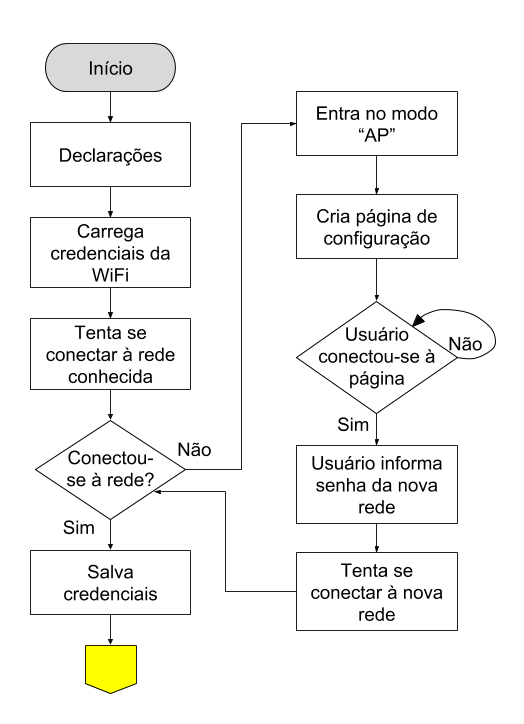
\includegraphics[width=0.4\textwidth]{figuras/flux_init.png}
    \end{center}
    \caption[Diagrama de fluxo da inicialização e conexão do sistema.]{Diagrama de fluxo da inicialização e conexão do sistema.}
    \label{finit}
\end{figure}

\subsubsection{\textit{Loop} Principal}

Antes de entrar no \textit{loop} principal são feitas as subscrições nos tópicos do protocolo MQTT. O programa então checa a conexão com o servidor e, caso não esteja conectado são feitas três tentativas de conexão e se não conseguir reconectar-se, o sistema é reiniciado. Após este passo, o programa espera por um tempo de cinco segundos por publicações nos tópicos subscritos, tais publicações são tratadas por rotinas específicas, chamadas de \textit{``callbacks''}, explicadas mais adiante. Caso o modo de funcionamento seja o ``Econômico'', o programa ajusta a intensidade com o controlador PID. Enfim a intensidade atual é publicada no tópico \texttt{``/pwmout''}, para que seja feito o acompanhamento do consumo, e volta a checar a conexão com o servidor completando um \textit{loop} de execução.

\begin{figure}[ht]
    \begin{center}
    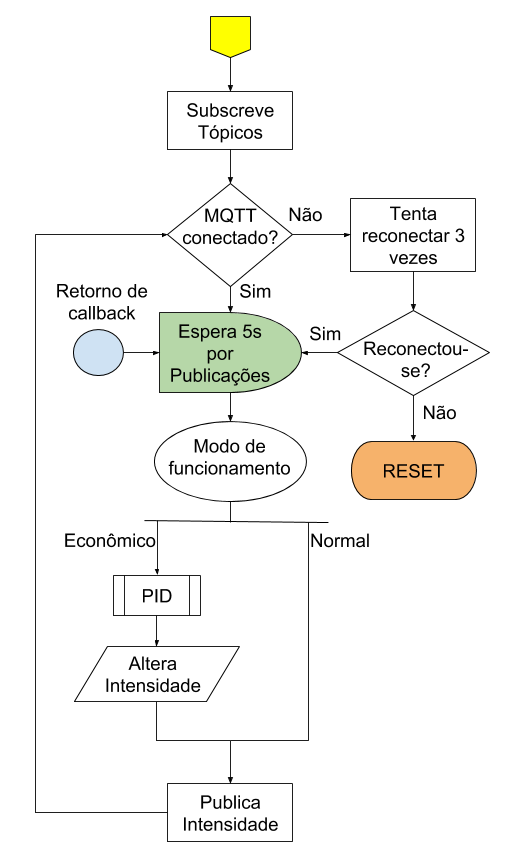
\includegraphics[width=0.4\textwidth]{figuras/flux_loop.png}
    \end{center}
    \caption[Diagrama de fluxo do ciclo de repetição principal do programa.]{Diagrama de fluxo do ciclo de repetição principal do programa.}
    \label{floop}
\end{figure}

\subsubsection{Rotinas de \textit{Callback}}

O \textit{loop} principal possui uma rotina de espera por publicações onde o programa monitora o servidor por publicações nos tópicos subscritos; tal rotina deve ser onde o programa passa a maior parte do tempo e caso uma publicação ocorra e o programa não esteja preparado, esta é perdida e só pode eventualmente ser recebida por reenvio da mensagem publicada (problema coberto nos níveis de QoS 1 e 2).

O recebimento de uma publicação desencadeia a execução de rotinas próprias de cada tópico subscrito, chamadas ``\textit{callbacks}''. Tais funções recebem os dados da publicação e os processa para definir o comportamento do sistema de iluminação e então retorna à rotina de espera de publicações.

A função de \textit{callback} do tópico ``\texttt{/onoff}'' recebe o dado na forma de texto (\textit{string}) que pode ter dois valores ``ON'' ou ``OFF'', no primeiro caso o sistema aplica a instensidade por PWM definida previamente e retorna, e no segundo caso o sistema desliga a iluminação aplicando intensidade nula e retorna. A função de \textit{callback} do tópico ``\texttt{/modo}'' tem como objetivo selecionar o modo de funcionamento (``Normal'' com ajuste manual ou ``Econômico'' com ajuste automático) e salvar a referência de iluminação (\textit{setpoint}) do modo automático de ajuste. A função de \textit{callback} do tópico ``\texttt{/pwmin}'' salva o dado de intensidade recebido, e caso o sistema já esteja ligado, aplica essa intensidade e salva o \textit{setpoint}, e então retorna.

\begin{figure}[ht]
    \begin{center}
    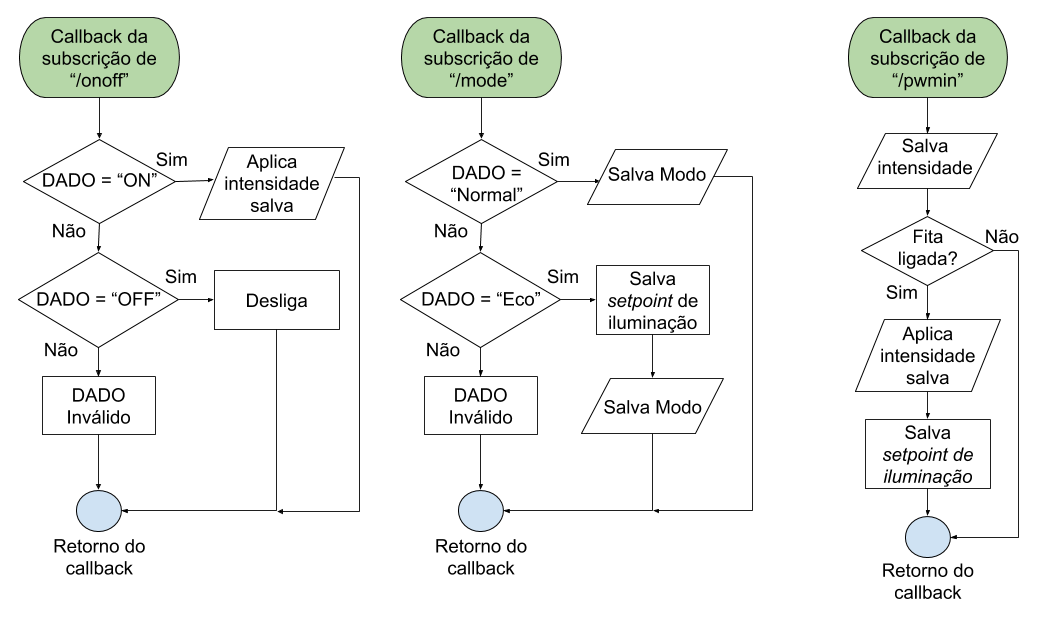
\includegraphics[width=0.8\textwidth]{figuras/flux_cb.png}
    \end{center}
    \caption[Diagrama de fluxo das rotinas de \textit{callback}.]{Diagrama de fluxo das rotinas de \textit{callback} dos tópicos ``\texttt{/onoff}'', ``\texttt{/pwmin}'' e ``\texttt{/modo}''.}
    \label{fcb}
\end{figure}

\subsection{Aplicativo Móvel}

A interface por aplicação móvel para sistemas \textit{Android} usada é baseada no aplicativo ``MQTT \textit{Dash}'', disponível, gratuitamente, na loja oficial da \textit{Google} \cite{dash}. O aplicativo permite várias interfaces independentes; ao criar uma interface, o usuário define várias características como nome da interface, endereço do servidor MQTT, o número da porta, nome de usuário, senha, e número de linhas e colunas do \textit{layout} da interface. Pode ser criado um atalho na tela inicial do aparelho da interface. Criada a interface o usuário pode criar elementos, denominados ``\textit{widgets}'', que podem ser botões, mostradores, e algumas estruturas que permitem escolher um número arbitrário em um intervalo, ou uma estrutura que permita a escolha de uma dentre múltiplas opções predefinidas. Os \textit{widgets} interagem na rede MQTT ao publicar mensagens escolhidas pelo usuário ou predefinidas no aplicativo, mostrar valores recebidos devido a subscrições, ou ainda apresentar determinados comportamentos dependendo da mensagem recebida ou publicada.

A interface criada para este projeto conta com três \textit{widgets}: Um botão para ligar e desligar a iluminação, uma estrutura para escolher um valor de 0 a 100 correspondente a porcentagem da intensidade da iluminação e uma estrutura que permite alternar entre os modos de funcionamento econômico ou normal. Os \textit{widgets} estão sincronizados com a interface \textit{web} por meio da subscrição nos mesmos tópicos em que publicam, isto significa que seu estado muda automaticamente caso haja publicação nesse mesmo tópico.

\begin{figure}[ht]
    \begin{center}
    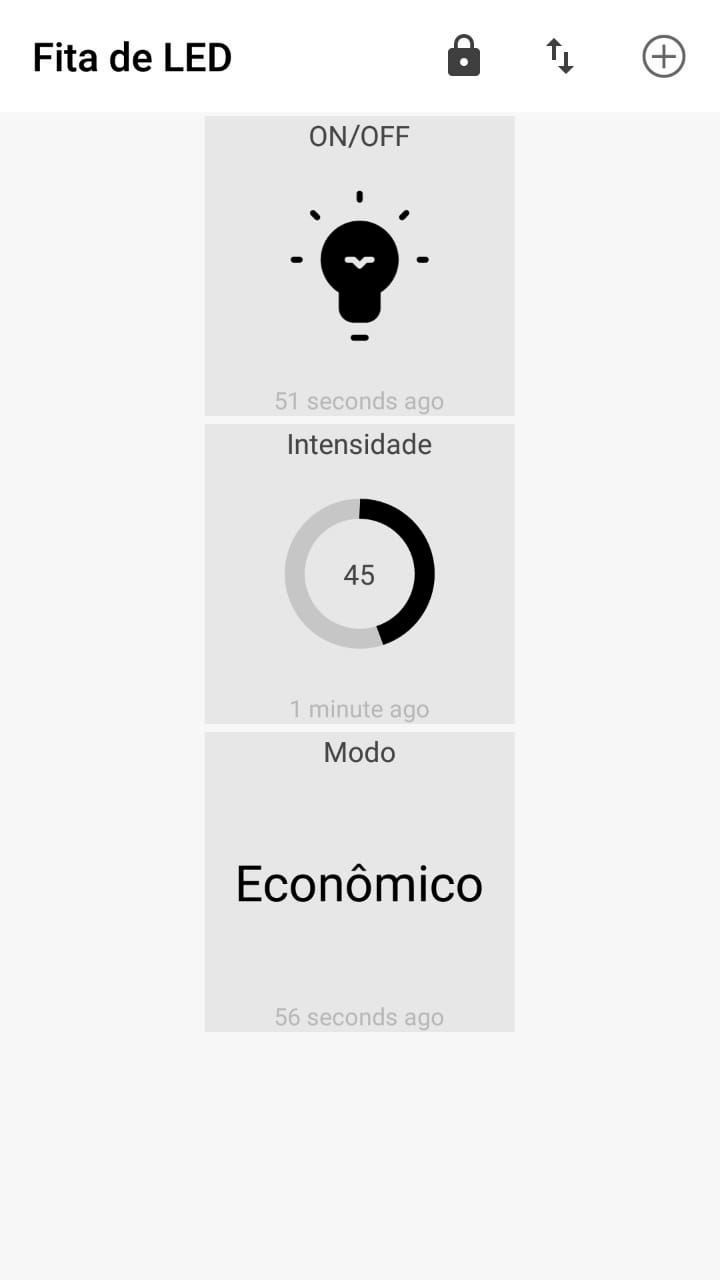
\includegraphics[width=0.4\textwidth]{figuras/appdash.png}
    \end{center}
    \caption[Ilustração do aplicativo móvel.]{Ilustração do aplicativo móvel com cores invertidas para evitar o fundo escuro da imagem.}
    \label{appdash}
\end{figure}

O botão ``ON/OFF'' pode ligar e desligar a iluminação ao publicar os valores ``ON'' e ``OFF'', respectivamente, no tópico ``\texttt{/onoff}'' e apresenta um visual lúdico: Quando se encontra no estado ON mostra a figura de uma ``lâmpada acesa'' e quando no estado OFF mostra a figura de uma ``lâmpada apagada''. 

A estrutura que permite arbitrar a intensidade da iluminação, chamado no aplicativo de ``\textit{slider}'', publica e subscreve no tópico ``\texttt{/pwmin}'' valores inteiros no intervalo de $0$ a $100$ representando a porcentagem da intensidade máxima. O \textit{widget} ``Modo'' publica no tópico ``\texttt{/modo}'' e serve para selecionar o modo de funcionamento dentre as opções ``Econômico'', e ``Normal''. 

\subsection{Interface \textit{Web}}

A interface \textit{web} é uma das funcionalidades ofertadas pelo serviço da \textit{Adafruit} e têm \textit{widgets} bem parecidos com os do aplicativo móvel; com uma diferença principal: Há um widget que plota um gráfico temporal dos valores publicados em algum dos tópicos e permite que os dados de qualquer tópico possam ser salvos em um arquivo ``csv'', formato compatível com os principais editores de planilhas.

\begin{figure}[ht]
    \begin{center}
    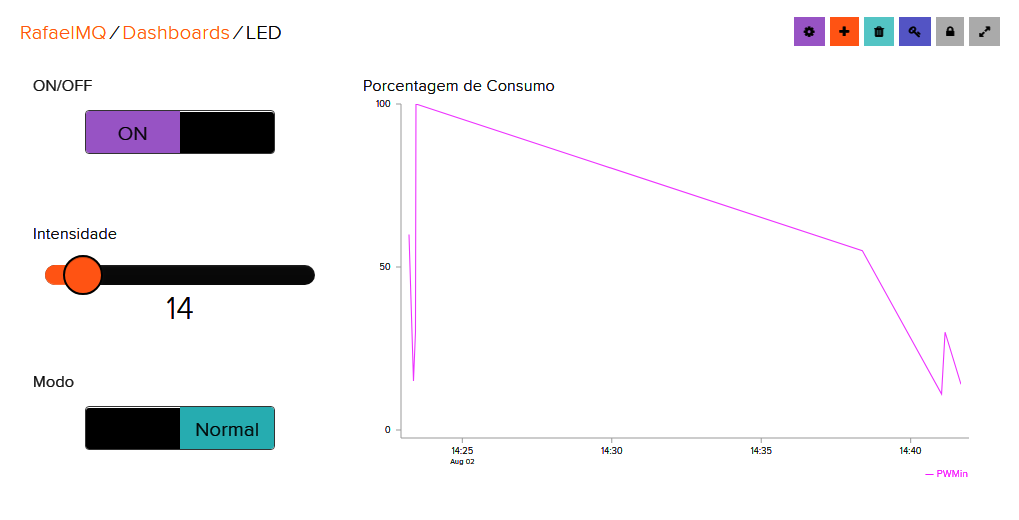
\includegraphics[width=\textwidth]{figuras/adaio.PNG}
    \end{center}
    \caption[Ilustração da interface \textit{web}.]{Ilustração da interface \textit{web} com cores invertidas para evitar o fundo escuro da imagem.}
    \label{adaio}
\end{figure}

O comportamento e funcionamento dos \textit{widgets} da interface \textit{web} é bastante similar ao dos \textit{widgets} da aplicação móvel com as mesmas estruturas de ligar e desligar, alterar a intensidade da iluminação e selecionar o modo de operação.

\subsection{Controle Automático de Luminosidade}

O controle automático de luminosidade é feito por uma malha fechada com um controlador PID digital no modo de funcionamento ``Econômico''. A referência do controlador \acf{PID} é definida como sendo a resistência do sensor de luminosidade no momento da ativação do modo econômico ou a partir da escolha da luminosidade desejada pelo usuário. O erro é calculado a cada iteração do programa como a diferença entre o valor de referência, ou \textit{setpoint}, e a  medida da resistência no sensor de luminosidade a cada iteração; e além do erro instantâneo, também são usados os valores de erro das duas últimas iterações segundo a equação \ref{eq:cd_12}. O tempo de amostragem é o tempo de execução de cada \textit{loop} do programa que consiste basicamente no tempo de espera por publicações.

O projeto de um controlador em malha fechada pode levar em conta diversas métricas de desempenho como tempo de estabilização, tempo de subida, magnitude de ``\textit{overshoot}'', classificação do amortecimento como subamortecido, sobreamortecido e criticamente amortecido, e alguns outros. Existem vários métodos de ajuste das constantes proporcional, derivativa e integral, alguns mais elaborados com métodos de otimização e outros mais simples como o método de ``tentativa e erro''. Para esse projeto será utilizada a abordagem de ``tentativa e erro'' de forma sistemática com o método de Ziegler-Nichols, com o objetivo principal de minimizar o erro no menor tempo possível, isto significa que os parâmetros serão ajustados para obter um baixo tempo de subida e estabilização.

Alguns ajustes são feitos em função das limitações do controlador: A luminosidade não pode ser controlada acima da capacidade máxima do sistema nem abaixo da capacidade mínima. Variações mínimas da luminosidade são ignoradas. Uma das não-linearidades conhecidas do sistema é a transformação da grandeza resistência elétrica do LDR, que varia com a luminosidade incidente sobre ele, e a tensão medida pelo microcontrolador sobre o divisor de tensão do LDR com o resistor fixo,
\begin{equation}
    \label{eq:prj1}
    V_{ADC} = C_{RES}\frac{R_{LDR}}{R_{LDR} + R_1}.
\end{equation}
Onde $V_{ADC}$ é o valor numérico da medição da tensão entregue pelo conversor, $R_{LDR}$ é a resistência do LDR, $R_1$ é o valor do resistor fixo do divisor de tensão e $C_{res}$ é a resolução do conversor analógico-digital, e no caso do conversor usado a resolução é de 1024 níveis, portanto os valores entregues pelo conversor serão números inteiros de 0 a 1023. Para contornar essa não-linearidade, o cálculo do valor da resistência do LDR, em função da tensão medida, é realizado em tempo de execução.
\begin{equation}
    \label{eq:prj1.1}
    R_{LDR} = \frac{V_{ADC}R_1}{C_{RES} - V_{ADC}}.
\end{equation}

Outro método usado para melhorar o desempenho do controlador foi o condicionamento do sinal de luminosidade medido, já que foi observado que mesmo ao medir luminosidade em situação bem estável, este apresentava um ruído de alta frequência que fazia a medição oscilar em torno de um valor médio. Para isso foi utilizador um filtro interpolador de duas medidas já que a maior parte do ruído é caracterizado pela alternância de valores em amostras consecutivas.
\begin{equation}
    \label{eq:prj2}
    H(z) = 0.5(1 + z^{-1}).
\end{equation}

Um outro típico ajuste usado em controladores PID consiste em limitar a componente integral do controle, que pode assumir valores altos quando o sistema começa a operar ou quando a referência muda bruscamente, efeito também conhecido como \textit{wind-up}. O efeito integral têm como objetivo principal o de eliminar o erro persistente em regime permanente, isto é, a componente constante do erro ao longo do tempo.

Os ajustes e sintonia descritos foram usados no desenvolvimento do algoritmo do controle de luminosidade. As sintonias típicas do método de Ziegler-Nichols serviram como ponto de partida para chegar a uma sintonia com valores aceitáveis de \textit{overshoot}, tempo de estabilização e amplitude de oscilação em regime permanente.